\documentclass{standalone}
\usepackage{tikz}
\usepackage{ctex,siunitx}
\setCJKmainfont{Noto Serif CJK SC}
\usepackage{tkz-euclide}
\usepackage{amsmath}
\usetikzlibrary{patterns, calc}
\usetikzlibrary {decorations.pathmorphing, decorations.pathreplacing, decorations.shapes,}

\begin{document}
\small
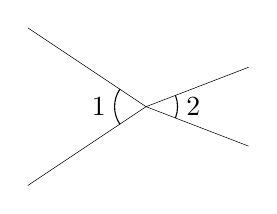
\begin{tikzpicture}[>=stealth,scale=1]
  \tkzSetUpPoint[fill=black]
  % \useasboundingbox(-1,-0.75)rectangle(3.7,1.4);
  \tkzDefPoints{0/1.5/O, -1.5/1.5+1/A, -1.5/1.5-1/B, 1.3/1.0/A', 1.3/2.0/B'}
  \tkzDrawSegments(A,O B,O A',O B',O)
  \tkzMarkAngles[mark=none, size=.4](A,O,B A',O,B')
  \tkzLabelAngle[pos=.6](A,O,B){1}
  \tkzLabelAngle[pos=.6](A',O,B'){2}
\end{tikzpicture}
\end{document}